\chapter{Implementation}
\chlab{implementation}

A system for fragment-based molecule parameterisation has three distinct tasks: visualising a molecule, finding matching fragments for that molecule, and allowing for interaction with the molecule and its matching fragments. As these tasks can be performed in isolation, it has been decided to implement the molecule parameterisation tool as three separate systems.

The front-end of the system, where users will carry out the parameterisation process, will be called the Online tool for Fragment-based Molecule Parameterisation~(\oframp). This name will also be used to refer to the system as a whole, as it is the hart of the system and is dependent on the other systems. The molecule is also visualised in \oframp, but the for this purpose essential, calculations of atom positions are done in the Online tool for Atom Position Calculations~(\oapoc). Finally, finding matching fragments and sorting them based on relevance is done by the Online tool for Molecule Fragment Finding~(\omfraf).

The complete network diagram for the fragment-based molecule parameterisation system is shown in \figref{diagram}. It is clear that \oframp{} is the central system, but that the more computation-intensive tasks are carried out by \oapoc{} and \omfraf{}. The remainder of this chapter will discuss each of the systems in more detail.


\begin{sidewaysfigure}[p]
\begin{center}
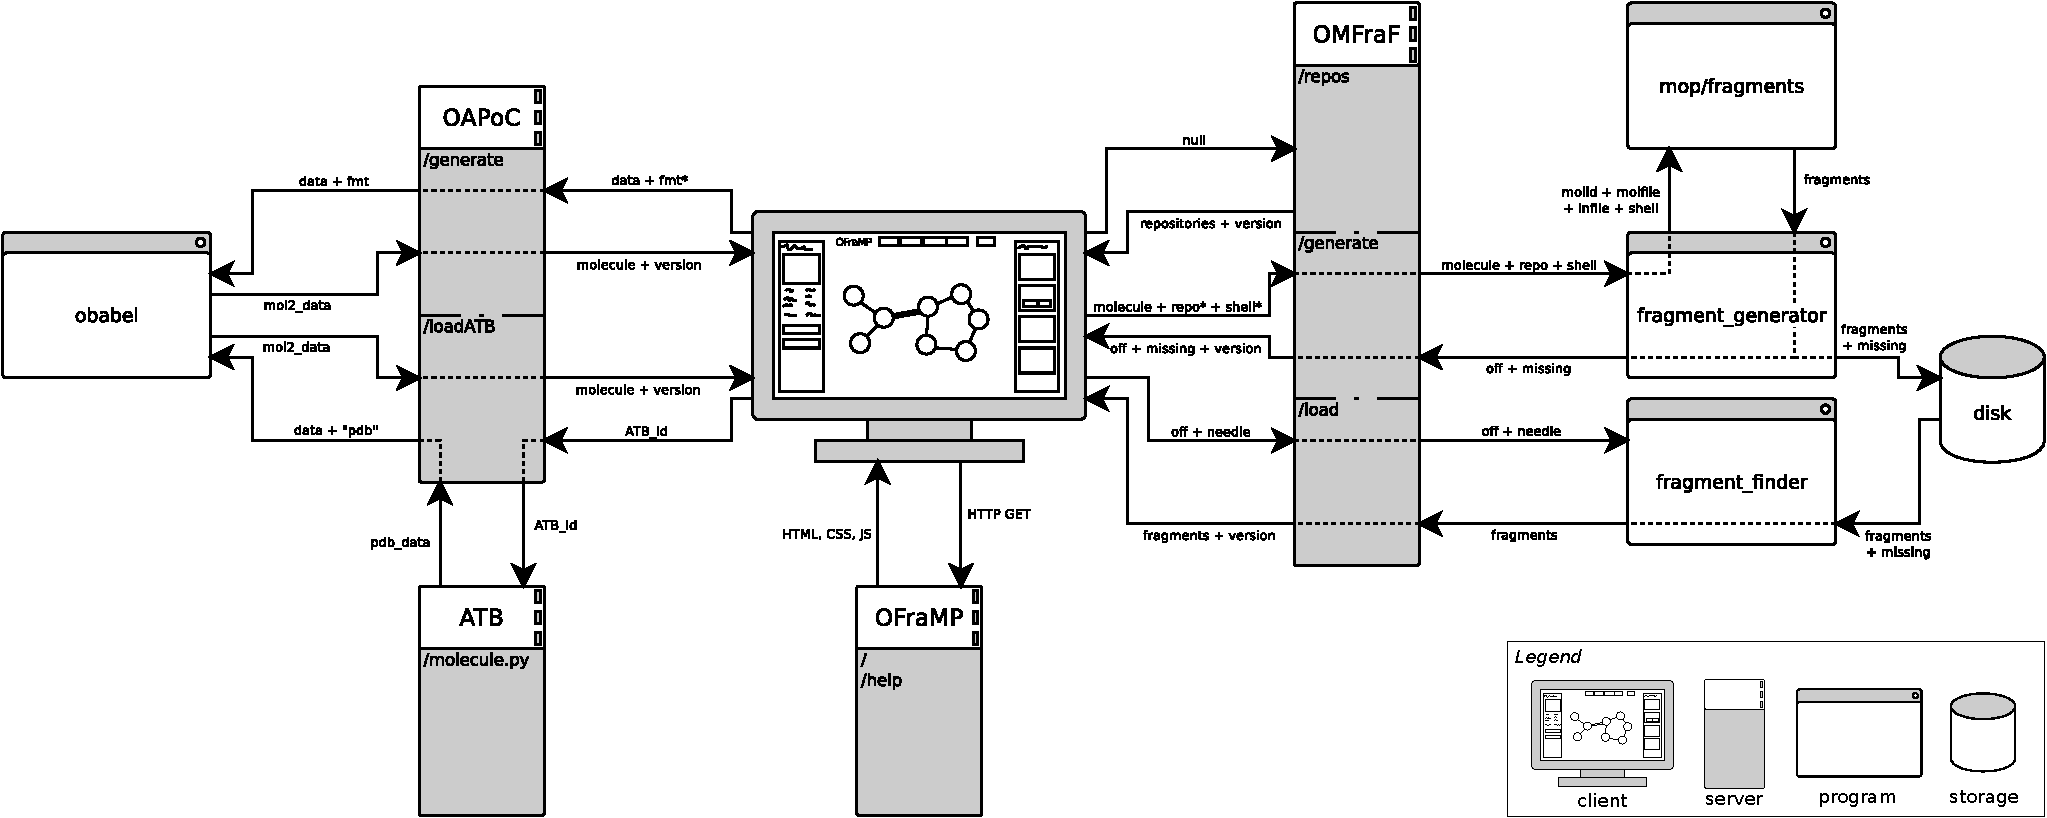
\includegraphics[width=\textwidth]{img/network_diagram.pdf}
\vspace{1em}
\caption{Network diagram of \oframp and its supporting systems.}
\figlab{diagram}
\end{center}
\end{sidewaysfigure}


\section[\oframp]{The Online tool for Fragment-based Molecule Parameterisation}
\oframp{} is the central part of the fragment-based molecule parameterisation system. It contains the user interface and connects with \oapoc{} and \omfraf{}. As discussed in \secref{platform}, it has been decided to implement the system as a web application. Following the current trend in web applications, \oframp{} has been implemented using the latest techniques from \verb|HTML5|, \verb|CSS3| and \verb|JavaScript|.

Using the latest web technologies allows for great cross-platform support. It allows the system to run on any desktop and laptop operating system, and creates the possibility of running it on a smartphone or tablet\footnote{This has not been a requirement for the project and has therefore not been tested extensively.}, without requiring any modifications. Still, of course, the limited size of a smartphone screen can be problematic, but it can at least run.

Making use of the latest \verb|HTML5| technologies, however, also comes at a cost. Older browsers generally lack support, and will therefore not be able to run \oframp. Luckily, according to the latest browser statistics from StatCounter~\cite{statcounter2014statcounter}, almost 85\% of internet users uses a browser that has full support for these technologies. Thanks to many compatibility libraries and especially the Internet Explorer \verb|canvas| fallback \verb|excanvas|~\cite{arvidsson2009explorercanvas}, partial support can be provided for browsers used by an additional 11\% of people. In total, this means that 96\% of internet users should be able to run \oframp. A complete list of system requirements can be found in \secref{client_req}.

\subsection{Getting started}

\begin{figure}[b!]
\begin{center}
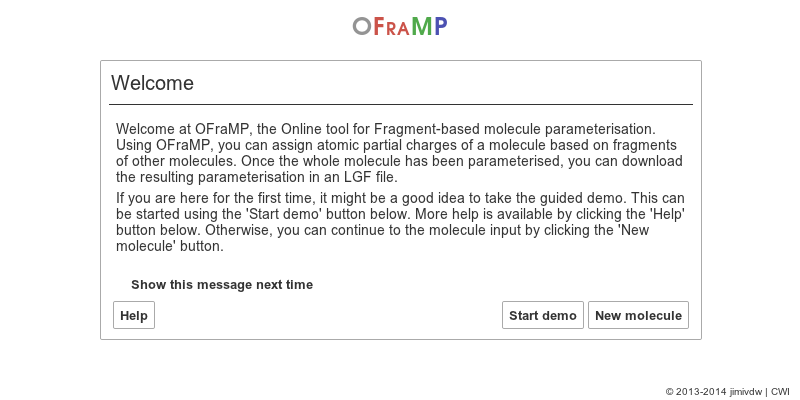
\includegraphics[width=.9\textwidth]{img/impl_welcome.png}
\caption{\oframp{} welcome screen.}
\figlab{impl_welcome}
\end{center}
\end{figure}

Upon loading \oframp{} for the first time, one should see something similar to what is shown in \figref{impl_welcome}. It is explained what the tool is, and what it should be used for. Additionally, instructions are provided for first-time users and pointers are provided to the help pages. From this point, users can either start a short demonstration guide~(see \secref{impl_demo}) or submit a new molecule into the system~(see \secref{impl_inserting}).

\Figref{impl_welcome} also shows the basic design of the system. It has been decided to go for a minimal look with a simple, purely textual logo. Besides the pastel colours of the logo, all text uses a dark shade of grey. Boxes and buttons all have a white background and a light grey, slightly rounded border.

Overly designed shiny elements are known to distract the user from his tasks~\cite{norman1990interfaces}~(see also \secref{design}). In some cases this may be beneficial, but for the purpose of finding a good molecule parameterisation this is undesirable. Therefore, this minimal design tries to make sure the user stays focused on the task that he needs to perform, rather than on using the tool. Furthermore, the tool still looks good and decent, which should prevent the users from distrusting it due to poor design~\cite{norman2002emotion}~(see also \secref{design}).

\subsubsection{Submitting a molecule}
\seclab{impl_inserting}

\begin{figure}[t!]
\begin{center}
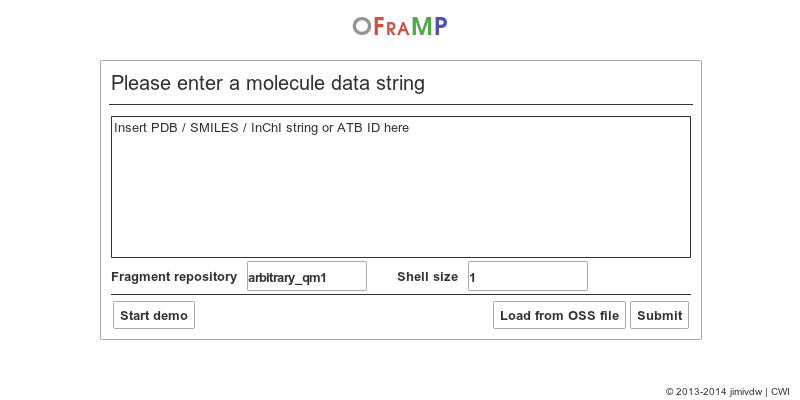
\includegraphics[width=.9\textwidth]{img/impl_inserting.png}
\caption{Insertion window for molecule data strings.}
\figlab{impl_inserting}
\end{center}
\end{figure}

In \figref{impl_inserting}, the insertion window for molecules is shown. This is where users should submit the molecules in a machine readable format, the so called molecule data string~(MDS). As discussed before, the system supports the \verb|PDB|, \verb|SMILES|, and \verb|InChI| formats, and the use of \verb|ATB ID|s~(see \secref{id_common}). When the MDS has been entered, the user can click the `Submit' button, after which the molecule will be displayed~(see \secref{impl_visualisation}).

Additionally, the user can adjust the fragment repository and shell size that are to be used for finding matching fragments of other molecules. This will be explained in more detail in \secref{impl_generating}. Furthermore, the demonstration mode~(see \secref{impl_demo}) can be started from this window as well, in case the user accidentally clicked the wrong button in the previous step. Finally, the user can load a so called \oframp{} State Storage~(OSS) file. These files can be created at any point in the parameterisation process and will store all progress up until that point. They can be loaded again at a later stage to continue the parameterisation process from that point.


\subsection{Visualisation}
\seclab{impl_visualisation}
\nlipsum

\subsection{Parameterisation}
We use LGF files~\cite{dezso2011lemon}\ldots

\begin{figure}[h!]
\begin{center}
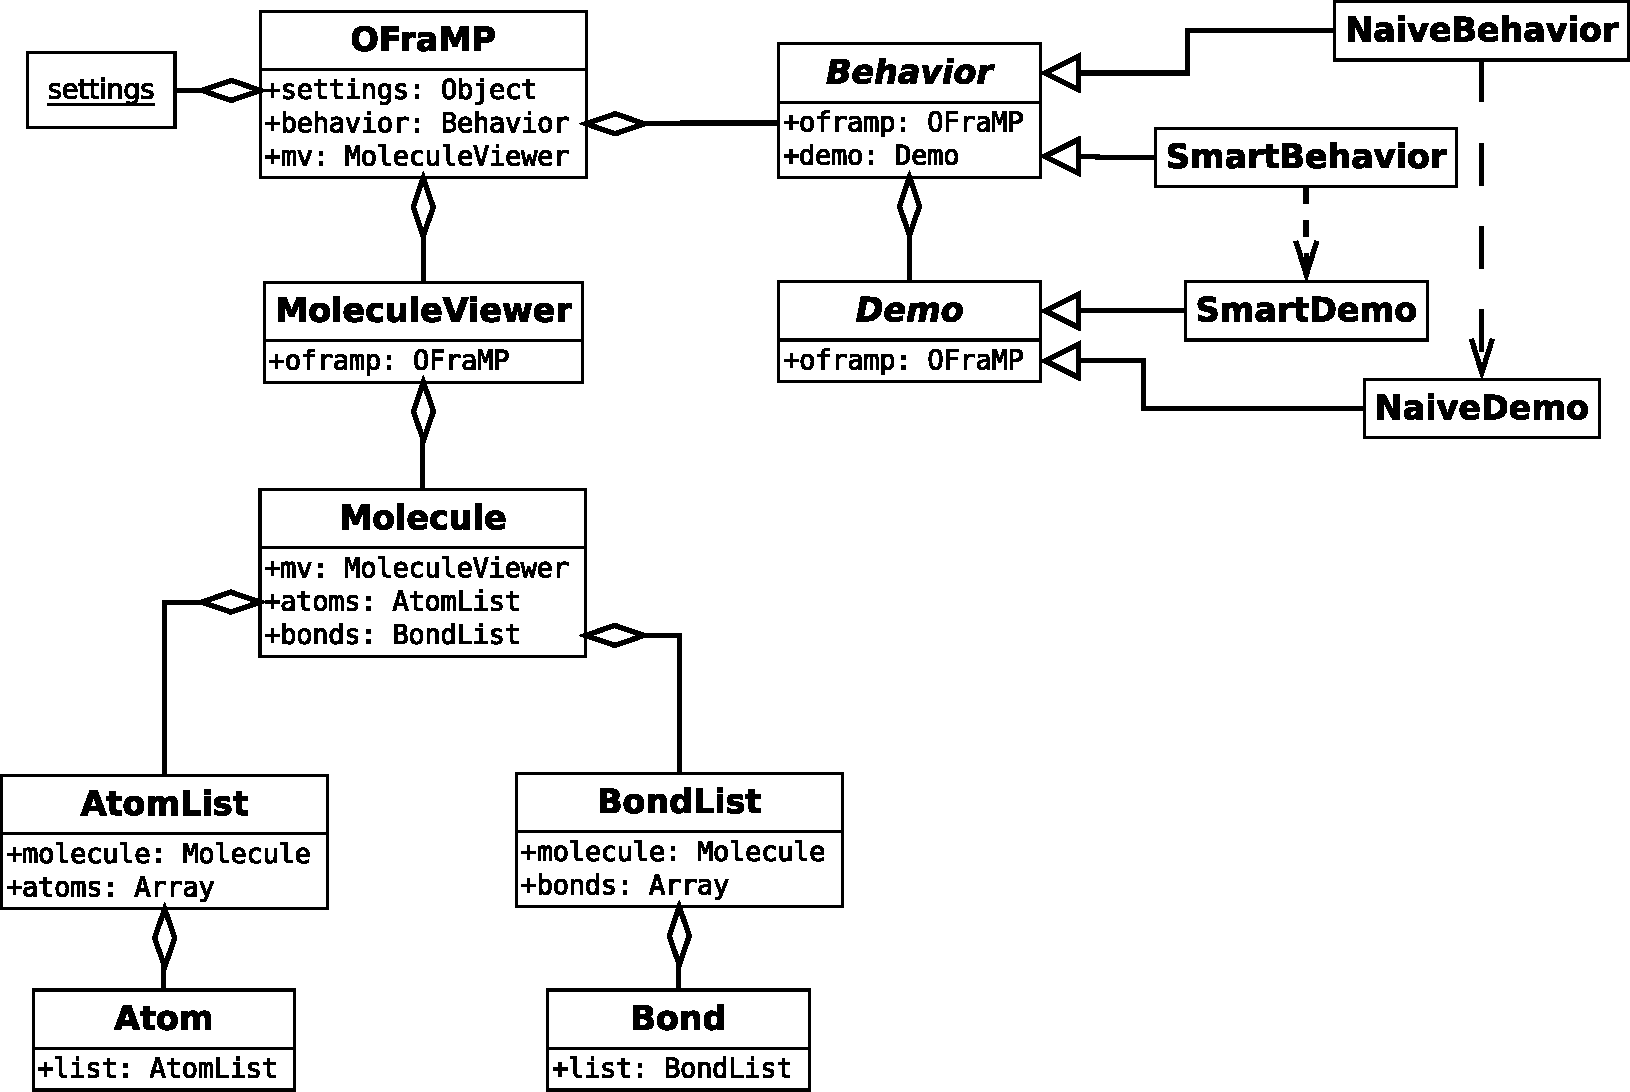
\includegraphics[width=\textwidth]{img/oframp_class.pdf}
\caption{Simplified class diagram of \oframp.}
\figlab{oframp_class}
\end{center}
\end{figure}

\nlipsum

\subsubsection{Manual `naive' version}
\nlipsum

\subsubsection{Semi-automatic `smart' version}
\nlipsum


\subsection{Fine-tuning charges}
\nlipsum


\subsection{Wrapping up}
\nlipsum


\subsection{Other features}
\nlipsum

\subsubsection{Demo mode}
\seclab{impl_demo}
\nlipsum

\subsubsection{Help}
\nlipsum

\subsubsection{Modifying visualisation parameters}
\nlipsum


\section[\oapoc]{The Online tool for Atom Position Calculations}
\nlipsum

\subsection{From ATB}
\nlipsum

\subsection{obabel}
\nlipsum


\section[\omfraf]{The Online tool for Molecule Fragment Finding}
\nlipsum

\subsection{Getting the repositories}
\nlipsum

\subsection{Generating fragments}
\seclab{impl_generating}
\nlipsum

\subsubsection{mop/fragments}
\nlipsum

\subsection{Finding fragments}
\nlipsum
